\section{Simulations}
In regards of the simulation scenarios we are deliberately neglecting the
critical aspects of the communication between master and slave, therefore
assuming ideal conditions as an istantaneous and loss-less signal trasfer,
without noise.
The table in fig describes the parameters chosen such as inertiae and
cut-off frequencies in addition to the range of values that the virtual
coefficients have undertaken.
% todo     correct from ubuntu
\begin{table}[H]
\centering
	\begin{tabular}{c c c c}
		\toprule
		% Symbol & Parameter & Value & Unit\\
		% \midrule 
		% \midrule 
    % & \textsl{Master-Slave manipulator}\\
		% \midrule 
		$J_{m}$  & Master Inertia & $5\cdot 10^{-4}$ & $kg\dot m^{2}$ \\
		$J_{s}$  & Slave Inertia & $5\cdot 10^{-4}$ & $kg\dot m^{2}$ \\
    % \midrule 
    % &\textsl{Desired cut-off frequencies}
		% \midrule 
		% $g_{1}$  & 1\textsuperscript{st} cut-off frequency & $5\cdot 10^{1}$ & rad/s \\
		% $g_{2}$  & 2\textsuperscript{nd} cut-off frequency & $5\cdot 10^{2}$ & rad/s \\
		% \midrule 
    % &\textsl{Virtual parameters}
		% \midrule 
    % $K_{v}$  & Spring stiffness & 2.5 - 20 & $N\,m/rad$\\
		% $B_{v}$  & Damping coefficient & $5.5\cdot 10^{-2}$ - $4.4\cdot 10^{-1}$ & $N\,m\,s/rad$\\
		% $J_{v}$  & Virtual inertia & $-\,4\cdot 10^{-4} -- 3\cdot 10^{-4}$& kgm\textsuperscript{2}\\
		\bottomrule
	\end{tabular}
	\caption{Parameters adopted in simulations}
	\label{simParams}
\end{table}

\subsection{Disturbance rejection performances}
As shows the bode diagram in fig different sets of virtual parameters
brings to different slope profile that will end up rejecting the
disturbances at higher frequencies than the cut-off ones.
Actually the corrispective values in Htz for the two cut-off frequencies are
respectively about 8 Htz and 80 Htz.

\begin{figure}[h]
	\centering
	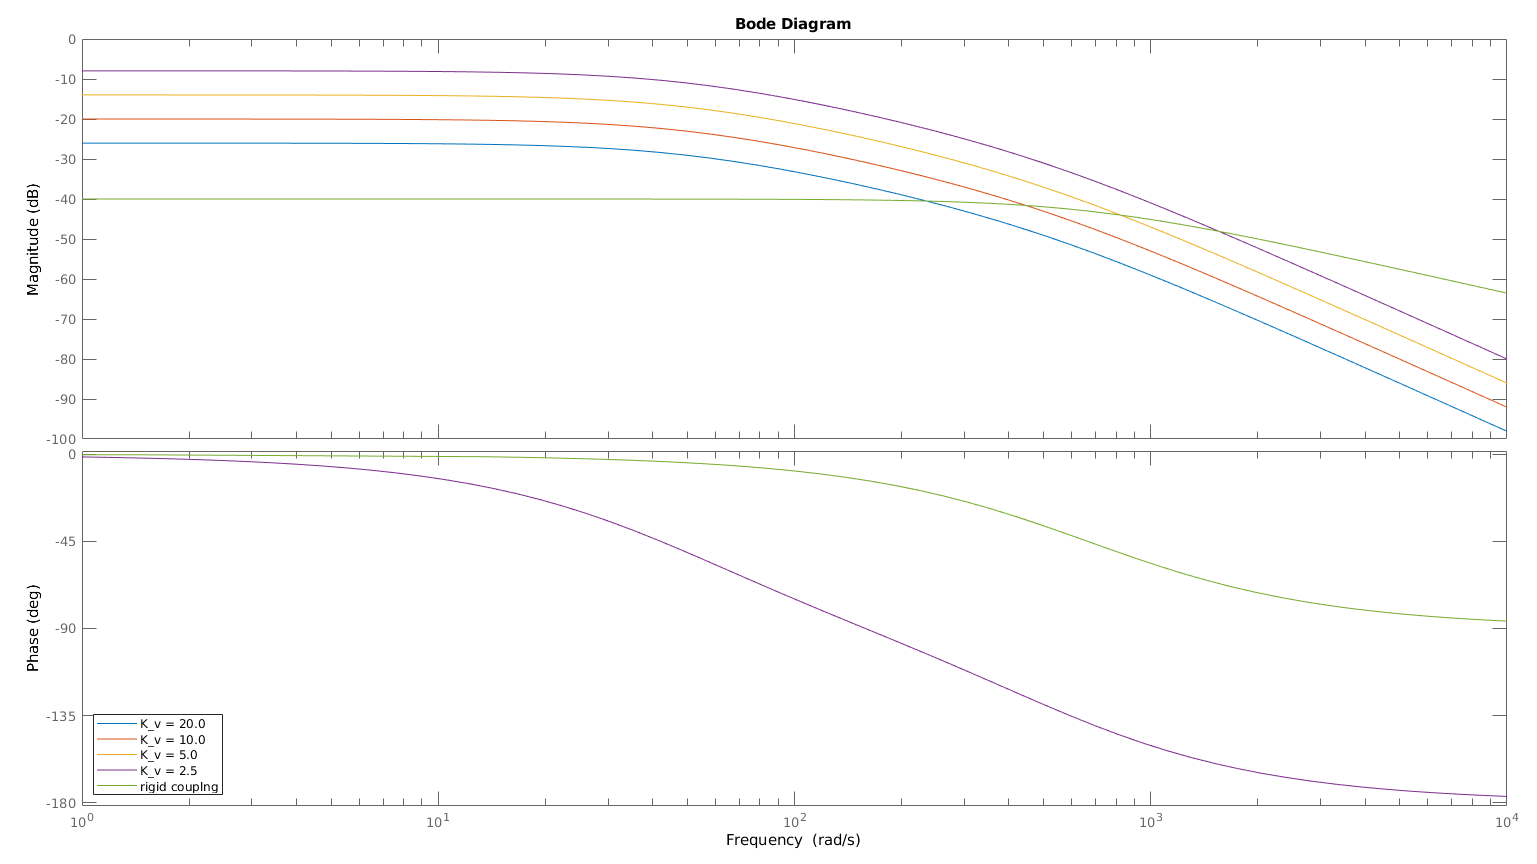
\includegraphics[width=1\linewidth]{Images/edoPics/bodo}
	\caption{bodo}
	\label{fig:bodo}
\end{figure}


In particular at frequencies higher than the cut-off frequencies, the
vibrations  due to a mixture of noises ( sinusoidal and white contribution ) will
be dumped more effectly by the sets of computed virtual parameters than in a rigid configuration.
In the rigid case full transparency is achieved betwen master and
slave thanks to a rather stiff interaction, this implies that the vibrations
generated slave-side will be felt almost with the same intensity whatever would
be the vibration frequency.
In fig is shown how the vibrations at lower frequencies are preserved by the
virtual sets, it is a rather desiderable aspect of a teleoperation interaction
since the input commands generated by the controller will have this kind of frequency.
Furthermore, as depicited by fig the vibrations that are more likely to belong
to environment noise ( high frequencies, in this case $10^3$ rad/sec ) are
filtered  out with greater efficency by the proposed virtual parameter sets than
in the rigid coupling behaviour.


\subsection{Task execution analisys}

At first, we present an execution in free motion where, as shown in fig, the
slave succeds to follow the trajectory given to the master, with almost no error
(without considering the noise ).

Then, in fig, the task will be divided in a freemotion part followed by an
enviromental contact after a certain angle of the slave.

\section{Results}